Este capítulo presenta las herramientas y tecnologías utilizadas en el desarrollo del proyecto. Se describen las características principales del microcontrolador ESP32, el lenguaje de programación C++ y el entorno de desarrollo integrado Arduino IDE.

\section{Microcontrolador ESP32 con OLED integrado}

El microcontrolador ESP32 con OLED integrado, específicamente el modelo ESP32 WiFi Kit 32 de Heltec, es una herramienta poderosa y versátil utilizada en el desarrollo de aplicaciones embebidas. Este microcontrolador combina las capacidades de conectividad del ESP32 con una pantalla OLED integrada, ofreciendo una plataforma compacta y eficiente para una amplia gama de proyectos.


\begin{figure}[!htb]
  \centering
   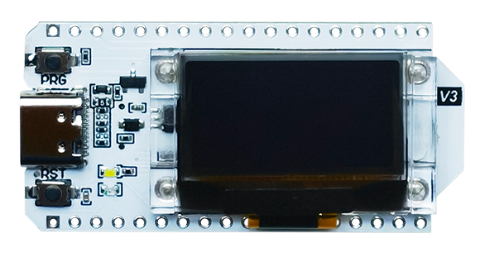
\includegraphics[width=0.25\linewidth]{figures/esp32heltec.png}
  \caption{Microcontrolador ESP32 con OLED integrado}
  \label{figure:esp32heltec}
\end{figure}
